
%%%%%%%%%%%%%%%%%%%%%%%%%%%%%%%%%%%%%%%%% 
% Short Sectioned Assignment
% LaTeX Template
% Version 1.0 (5/5/12)
% 
% This template has been downloaded from:
% http://www.LaTeXTemplates.com
% 
% Original author:
% Frits Wenneker (http://www.howtotex.com)
% 
% License:
% CC BY-NC-SA 3.0 (http://creativecommons.org/licenses/by-nc-sa/3.0/)
% 
%%%%%%%%%%%%%%%%%%%%%%%%%%%%%%%%%%%%%%%%% 

% ----------------------------------------------------------------------------------------
% PACKAGES AND OTHER DOCUMENT CONFIGURATIONS
% ----------------------------------------------------------------------------------------

\documentclass[paper=letter, fontsize=11pt]{scrartcl} % A4 paper and 11pt font size

\usepackage[T1]{fontenc} % Use 8-bit encoding that has 256 glyphs
\usepackage{fouriernc} % Use the Adobe Utopia font for the document - comment this line to return to the LaTeX default
\usepackage[english]{babel} % English language/hyphenation
\usepackage{amsmath,amsfonts,amsthm} % Math packages
\usepackage{bm}
\usepackage{graphicx}
\usepackage{siunitx}
\usepackage{sectsty} % Allows customizing section commands
\renewcommand{\thesubsection}{(\alph{subsection})}
\sectionfont{\bfseries\rmfamily}
\subsectionfont{\rmfamily\normalfont\itshape}
%\allsectionsfont{\centering \normalfont\scshape} % Make all sections centered, the default font and small caps
\usepackage{fancyhdr} % Custom headers and footers
\pagestyle{fancyplain} % Makes all pages in the document conform to the custom headers and footers
\fancyhead{} % No page header - if you want one, create it in the same way as the footers below
\fancyfoot[L]{} % Empty left footer
\fancyfoot[C]{} % Empty center footer
\fancyfoot[R]{\thepage} % Page numbering for right footer
\renewcommand{\headrulewidth}{0pt} % Remove header underlines
\renewcommand{\footrulewidth}{0pt} % Remove footer underlines
\setlength{\headheight}{13.6pt} % Customize the height of the header
\usepackage[procnames]{listings}
\usepackage{color}
\usepackage[dvipsnames]{xcolor}
\usepackage[final]{pdfpages}
\definecolor{keywords}{RGB}{255,0,90}
\definecolor{comments}{RGB}{113,113,113}
\definecolor{red}{RGB}{160,0,0}
\definecolor{green}{RGB}{0,150,0}
 
\lstset{language=Python, 
        basicstyle=\ttfamily\small, 
        keywordstyle=\color{keywords},
        commentstyle=\color{comments},
        stringstyle=\color{red},
        showstringspaces=false,
        procnamekeys={def,class}}
      
% \numberwithin{equation}{section} % Number equations within sections (i.e. 1.1, 1.2, 2.1, 2.2 instead of 1, 2, 3, 4)
% \numberwithin{figure}{section} % Number figures within sections (i.e. 1.1, 1.2, 2.1, 2.2 instead of 1, 2, 3, 4)
% \numberwithin{table}{section} % Number tables within sections (i.e. 1.1, 1.2, 2.1, 2.2 instead of 1, 2, 3, 4)

\setlength\parindent{0pt} % Removes all indentation from paragraphs - comment this line for an assignment with lots of text

% ----------------------------------------------------------------------------------------
% TITLE SECTION
% ----------------------------------------------------------------------------------------

\newcommand{\horrule}[1]{\rule{\linewidth}{#1}} % Create horizontal rule command with 1 argument of height

\title{ 
  \normalfont \normalsize 
  \textsc{} \\ [25pt] % Your university, school and/or department name(s)
  \horrule{0.5pt} \\ [0.4cm] % Thin top horizontal rule
  \huge ASTR513 Homework2 \\ % The assignment title
  \horrule{2pt} \\ [0.5cm] % Thick bottom horizontal rule
}
\author{Joshua Lothringer, Yifan Zhou} % Your name
\date{\normalsize\today} % Today's date or a custom date

\begin{document}
\maketitle % Print the title

\section{From measurements to inferences}
In class, we studied the problem of projectile motion in a vertical,
uniform gravitational field $\vec{g}$ for which we want to infer the two
components of the initial velocity vector of the projectile, $u_{x}$ and $u_{y}$
given a measurement of the height h and range R of the motion. Repeat
this investigation in this homework problem with the additional
complication that our knowledge of the magnitude of the gravitational
field is not perfect.

In particular, assume that the uncertainties in our measurements of
the height and range of the projectile are well approximated by
Gaussian functions with means and standard deviations of
($h_{0} = \SI{1.0}{m}, \sigma_{h} = \SI{0.2}{m}$) and
($R_{0} = \SI{10.0}{m}, \sigma_{R} = \SI{0.2}{m}$), respectively. Also
assume that the uncertainty in our knowledge of the magnitude of the
gravitational field is also well described by a Gaussian with a mean
and standard deviation of
($g_{0} = \SI{9.81} {m s^{-2}}, \sigma_{g} = \SI{0.05}{m s^{-2}}$).

\subsection{follow the traditional approach to error propagation to
  infer the uncertainties in the inference of $u_{x}$ and $u_{y}$, given the
  measurement uncertainties.}

\begin{align}
u_x &= \sqrt{\frac{g}{2h}}\frac{R}{2}\\
u_y &= \sqrt{2gh}
\end{align}
Using error propagation
\newcommand{\dd}{\ensuremath{\mathrm{d}}}
\newcommand{\ddfrac}[2]{\ensuremath{\frac{\mathrm{d} #1}{\mathrm{d} #2}}}
\newcommand{\ppfrac}[2]{\ensuremath{\frac{\partial #1}{\partial #2}}}
\begin{align}
  \sigma_{u_{x}}^{2} &=\frac{g}{8h} \sigma_{R}^{2} +
                       \frac{R^{2}}{32gh}\sigma_{g}^{2} +
                       \frac{gR^{2}}{32h^{3}} \sigma_{h}^{2} \\
  \sigma_{u_{y}}^{2} &= \frac{h}{2g} \sigma_{g}^{2}  + \frac{g}{2h} \sigma_{h}^{2}
\end{align}

Thus
\begin{align}
  \sigma_{u_{x}} &= \SI{1.13}{ms^{-1}}\\
  \sigma_{u_{y}} &=\SI{0.43}{ms^{-1}}
\end{align}

\subsection{Following frequentist arguments, use Monte Carlo
  realizations of the three measurements ($h, R, \hbox{and}\,g$) based
  on the distribution of their uncertainties to investigate the
  correlation in the uncertainties of the inferred quantities
  ($u_{x}\, \hbox{and}\, u_{y}$). Use the same Monte Carlo realizations to
  generate the one-dimensional, marginalized distributions over ux and
  uy and compare them to the results of part (a).}

\newcommand{\ux}{\ensuremath{u_x}}
\newcommand{\uy}{\ensuremath{u_y}}
Monte Carlo result is presented in Figure \ref{fig:2b}. $u_{x}$ and
$u_{y}$ are tightly correlated. From the marginal distribution of
$u_{x}$ and $u_{y}$, \ux{} is skewed to large velocity, and \uy{} is
skewed to small velocity.
\begin{figure}
  \centering
  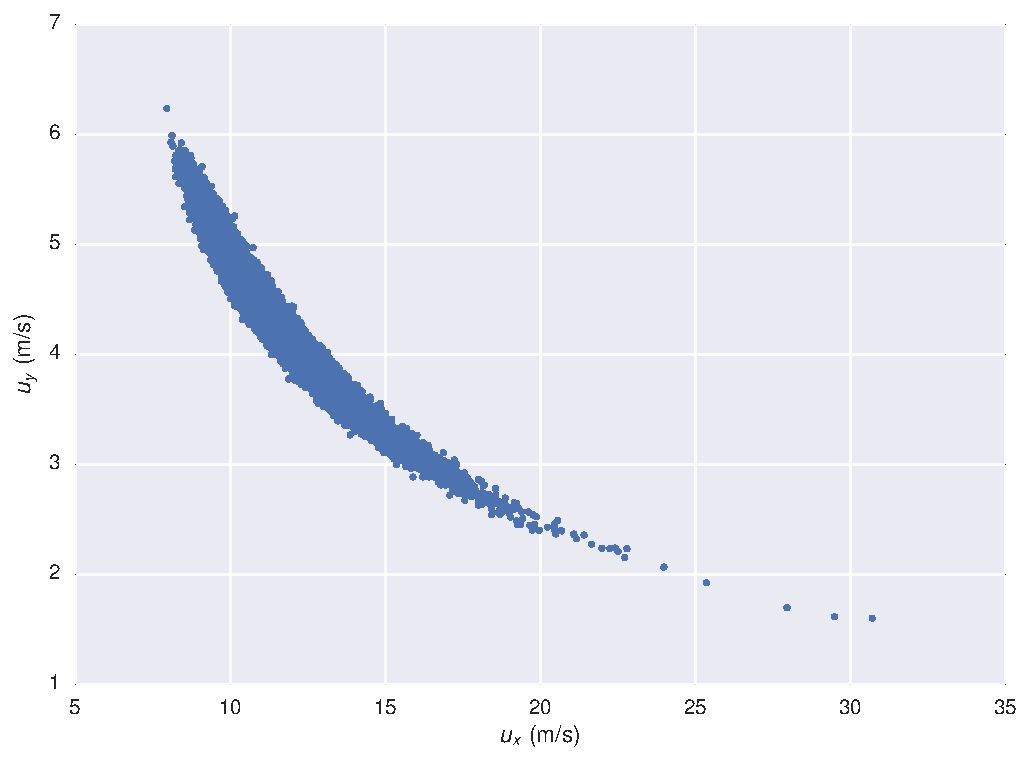
\includegraphics[width=0.8\textwidth]{MC_joint}\\
  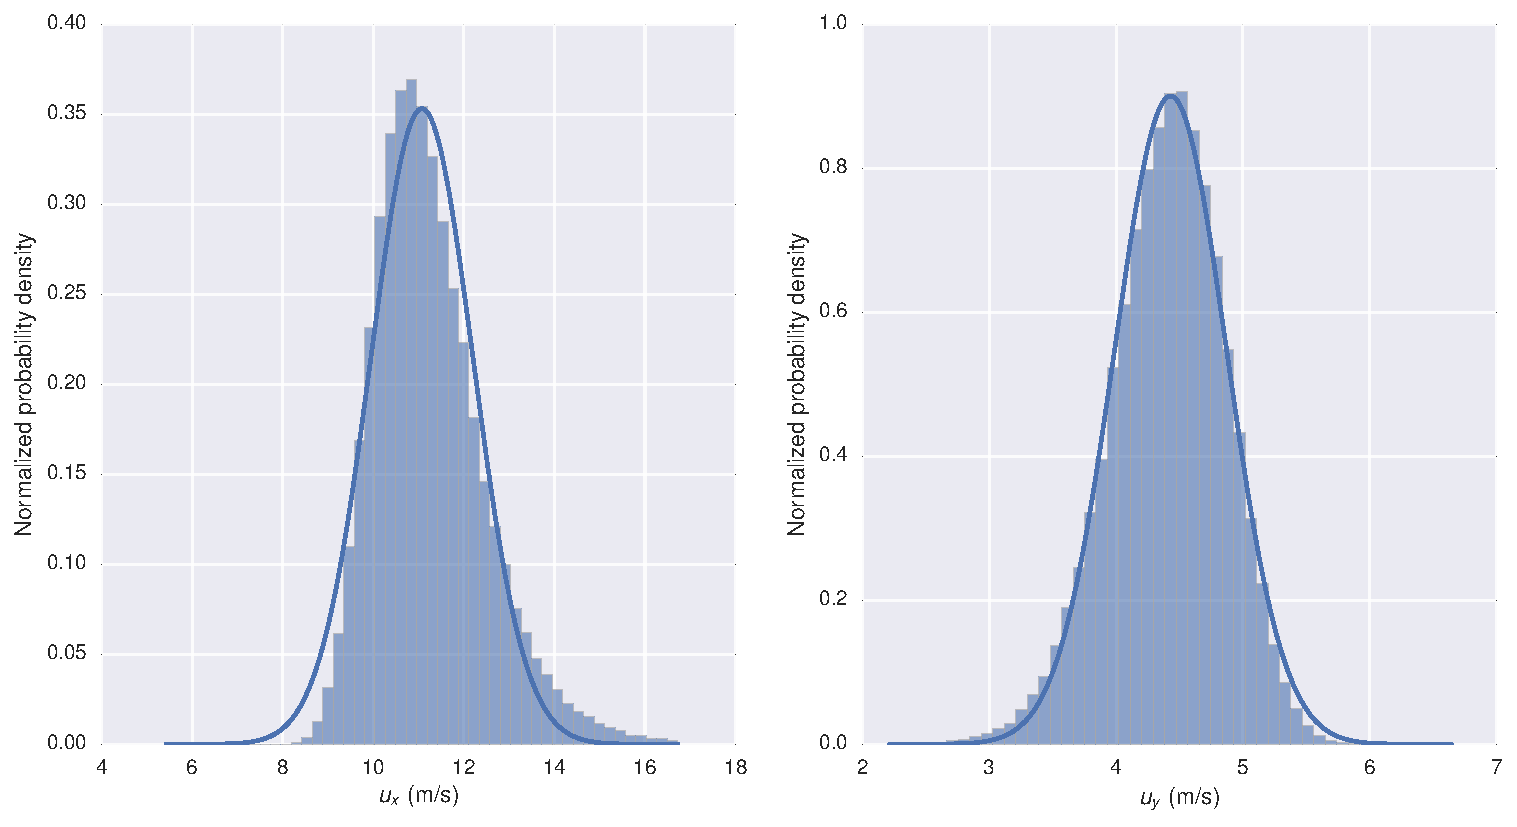
\includegraphics[width=\textwidth]{MC_MarginDist}
  \caption{Joint distribution and marginal distributions of $u_{x}$,
    and $u_{y}$.}
  \label{fig:2b}
\end{figure}

\subsection{ Repeat part (b) analytically using (Jacobian)
  transformations of the probability distributions of the
  measurement. Compare your results to the Monte Carlo simulations.}
\newcommand{\gaussian}[1]{\ensuremath{G(#1, \sigma_{#1})}}
\begin{equation}
  P(\ux, \uy, g) \dd\ux \dd\uy \dd g =
  \gaussian{h}\gaussian{R}\gaussian{g} \dd h \dd R \dd g
\end{equation}
\begin{equation}
  P(\ux, \uy, g) = \gaussian{h}\gaussian{R}\gaussian{g}
  \biggl|J\biggl(\frac{h, R, g}{\ux, \uy, g}\biggr)\biggr|
\end{equation}
Calculate the Jacobian determinant $J\biggl(\frac{h, R, g}{\ux, \uy,
  g}\biggr)$
\newcommand{\pfrac}[2]{\ensuremath{\frac{\partial #1}{\partial #2}}}
\begin{equation}
  \begin{split}
    J\biggl(\frac{h, R, g}{\ux, \uy,g}\biggr) &=
    \begin{vmatrix}
      \pfrac{h}{\ux}& \pfrac{h}{\uy} &\pfrac{h}{g}\\
      \pfrac{R}{\ux}& \pfrac{R}{\uy} &\pfrac{R}{g}\\
      \pfrac{g}{\ux}& \pfrac{g}{\uy} &\pfrac{g}{g}\\
    \end{vmatrix}\\
    & = -\frac{2\uy^{2}}{g^{2}}
  \end{split}
\end{equation}
\begin{equation}
  P(\ux, \uy, g) = \gaussian{h}\gaussian{R}\gaussian{g} \,\frac{2\uy^{2}}{g^{2}}
\end{equation}
Using numerical Integration to calculate $P(\ux)$ and $P(\uy)$:
\begin{align}
  P(\ux) &= \int \dd\uy \int\dd g P(\ux, \uy, g)\\
   P(\uy) &= \int \dd\ux \int\dd g P(\ux, \uy, g)
\end{align}
Plot the two semi-analitical result with Monte Carlo realization
(Figure \ref{fig:Jacobian}). Analytical calculation gives identical
results to MC realization.
\begin{figure}[!ht]
  \centering
  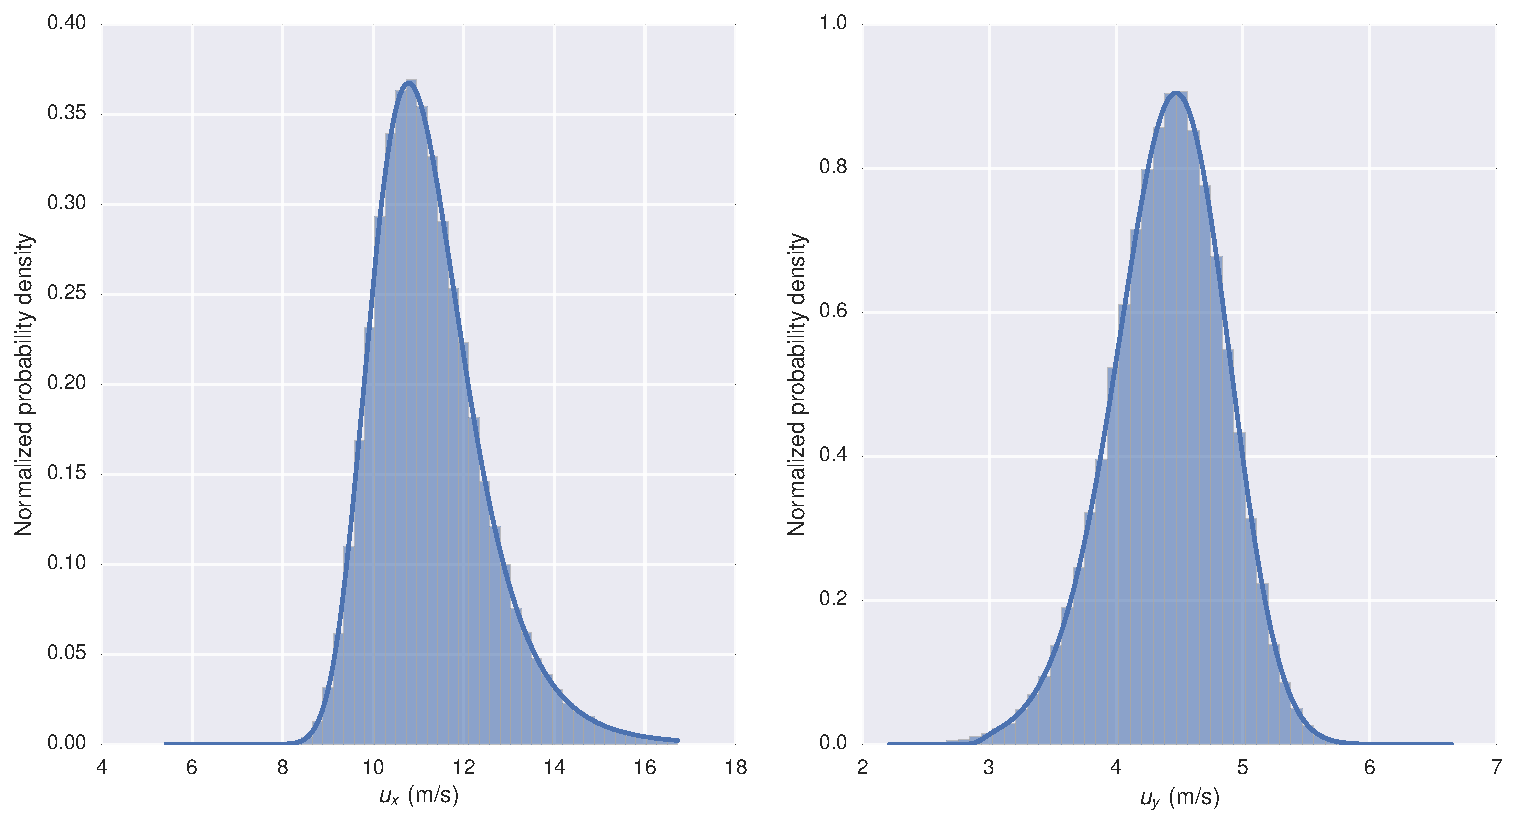
\includegraphics[width=\textwidth]{MC_Jacobian}
  \caption{Compare MC realization and analytical calculation using
    Jacobian transformation}
  \label{fig:Jacobian}
\end{figure}
\subsection{Solve the same problem using Bayesian arguments and
  compare the results to that of the frequentist approach. As a first
  attempt, use priors over ux and uy that are constant.}

\subsection{Explore the dependence of your Bayesian inferences on your
  priors. In particular, compare results with priors that are
  constant (e.g., as in part (d)) to those with logarithmic priors,
  i.e., $P_{\mathrm{pr}}(u_{x}) \sim u^{-1}$ and
  $P_{\mathrm{pr}}(u_{y}) \sim u^{-1}$.}
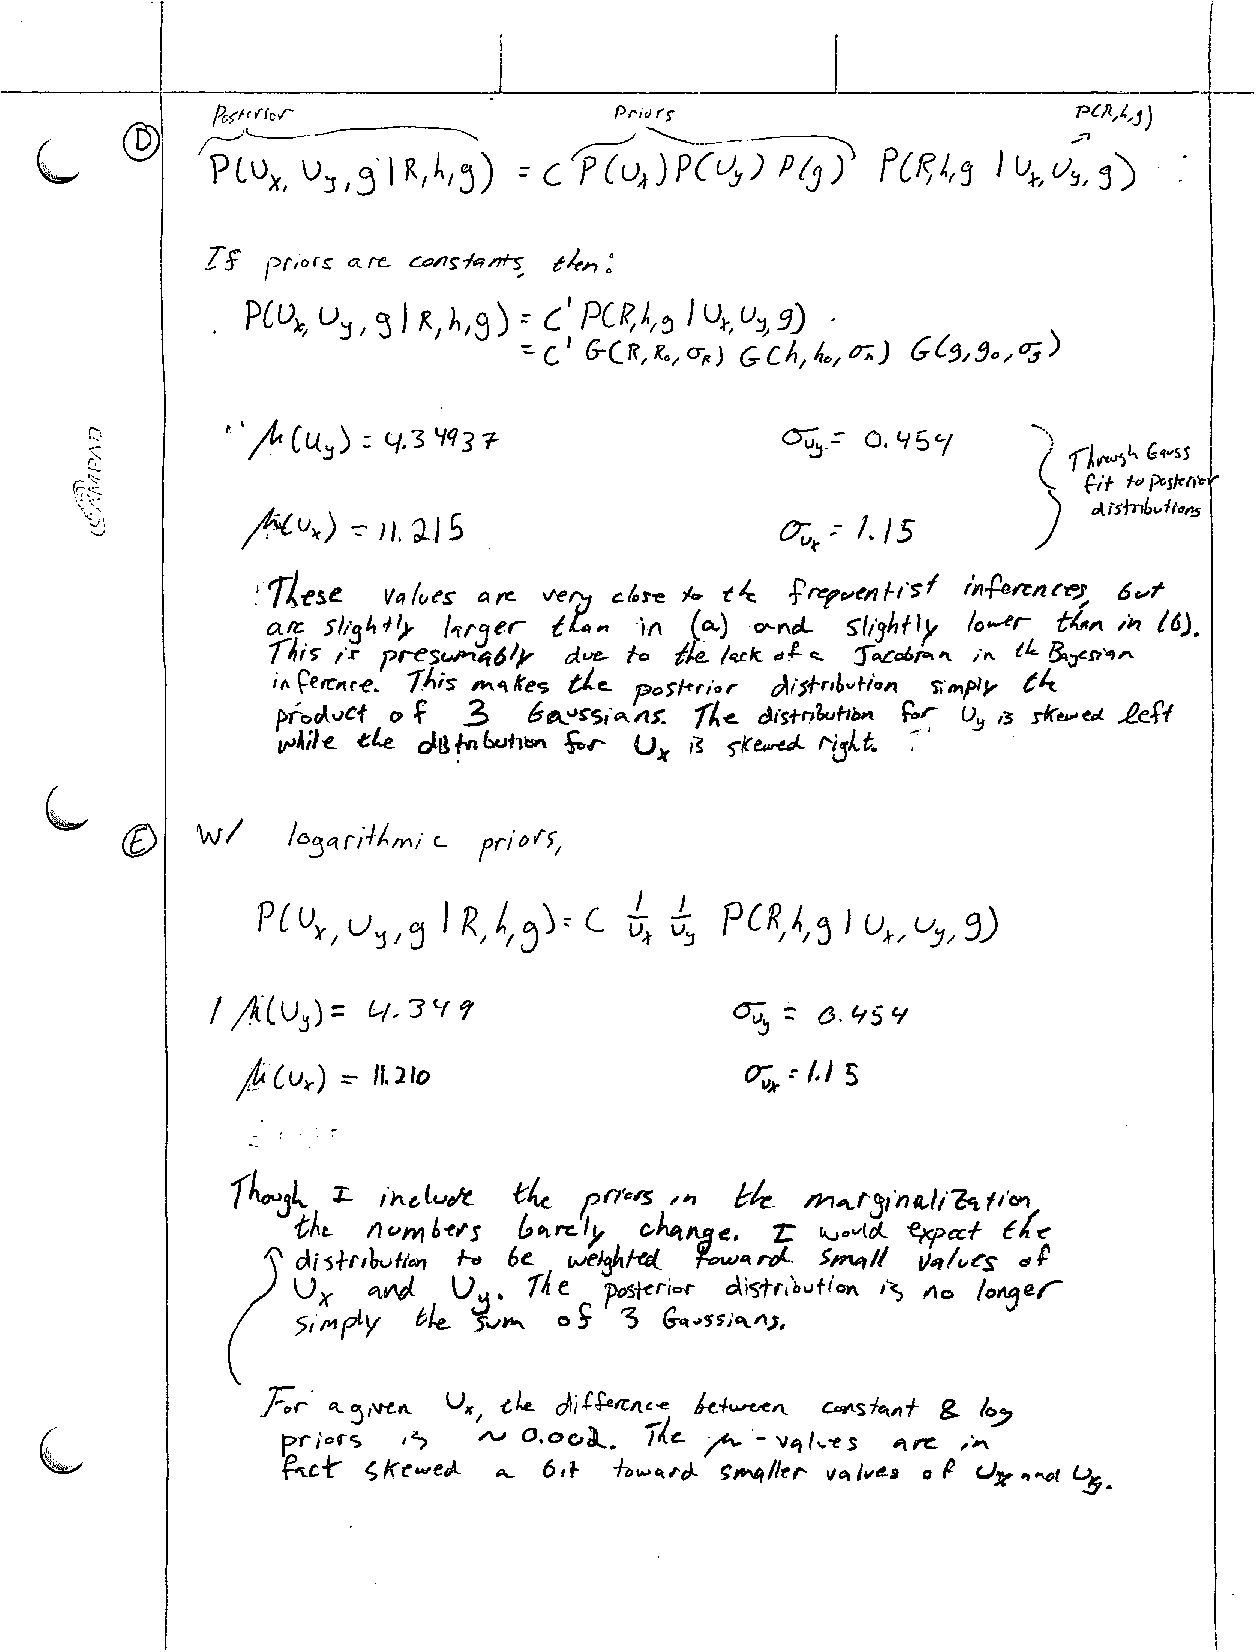
\includepdf{stats_hw2_de.pdf}
Figure \ref{fig:Bayesian} compares bayesian calculation, two kinds of
priors give very close results. Figure \ref{fig:compBayes} compares
the difference in detail.

\begin{figure}[!ht]
  \centering
  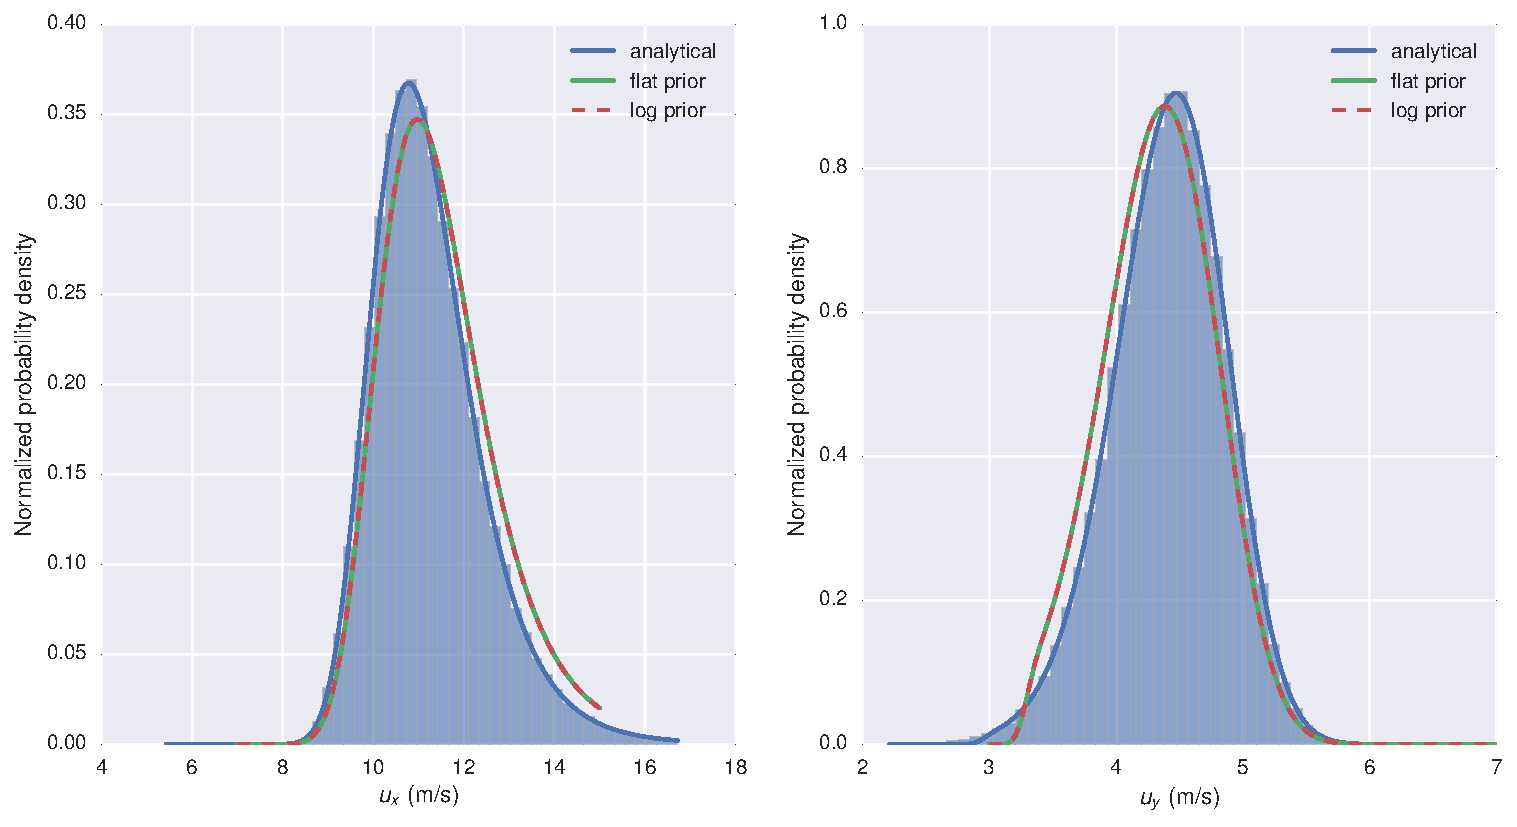
\includegraphics[width=\textwidth]{MC_Bayesian}
  \caption{Comparison of Bayesian results and analytical results}
  \label{fig:Bayesian}
\end{figure}

\begin{figure}[!ht]
  \centering
  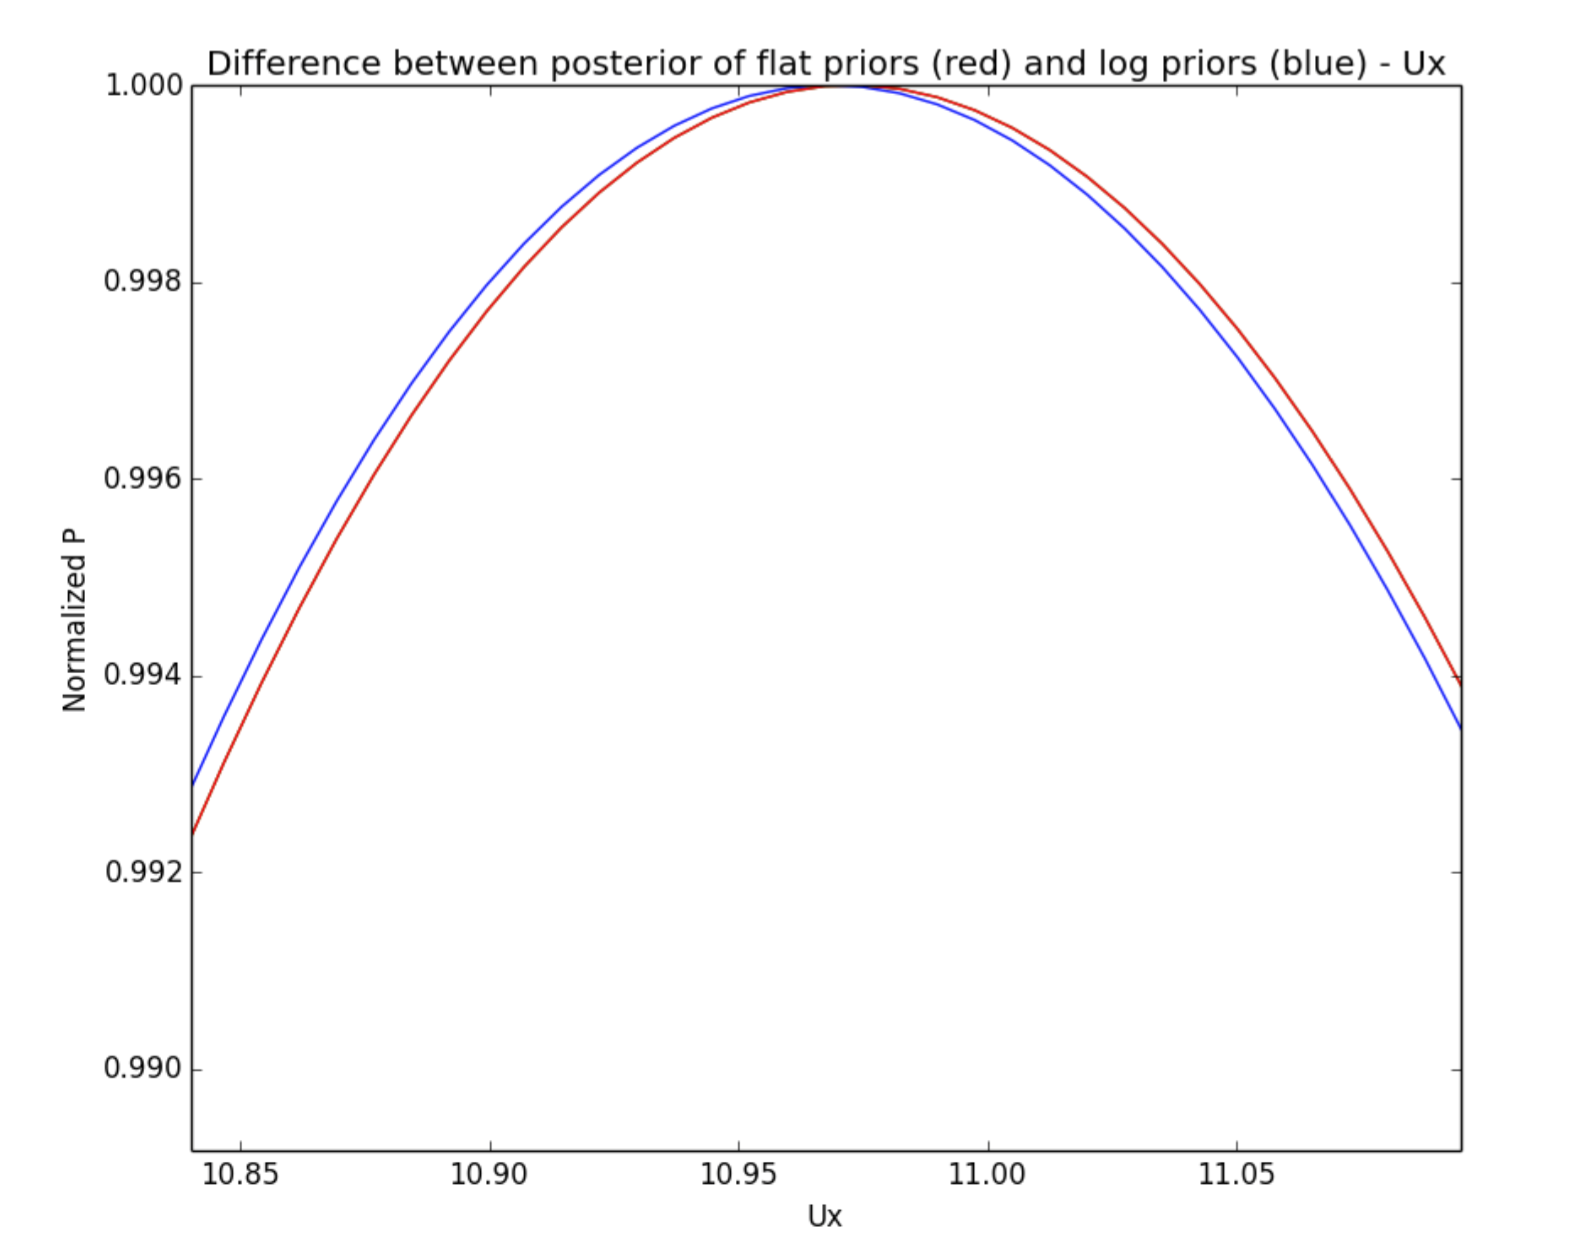
\includegraphics[width=0.6\textwidth]{prior_comp}
  \caption{Comparison of affects of different priors on $u_{x}$}
  \label{fig:Bayesian}
\end{figure}
\appendix{}
Code to compute the numerical integration.
\begin{lstlisting}
import numpy as np
from scipy.integrate import dblquad
def dPux(g, uy, ux):
    h0 = 1.0
    dh = 0.2
    R0 = 10
    dR = 0.2
    g0 = 9.81
    dg = 0.05
    C = 1 / ((2 * np.pi)**(1.5)* dR * dh * dg) * 2 * uy**2 / g**2
    exp1 = np.exp(-(uy**2 / (2 * g) - h0)**2/(2 * dh**2))
    exp2 = np.exp(-(2 * ux * uy / g - R0)**2/(2 * dR**2))
    exp3 = np.exp(-(g - g0)**2/(2 * dg**2))
    return C * exp1 * exp2 * exp3

def Pux(ux):
    """
    numerical integration
    """
    # integration limit defined by 5 sigma limit
    return dblquad(lambda g, uy: dPux(g, uy, ux),
                  2.21, 6.64,
                  lambda g: 9.56,
                  lambda g: 10.06,
                  )

def Puy(uy):
    return dblquad(lambda g, ux: dPux(g, uy, ux),
                  5.42, 16.72,
                  lambda g: 9.56,
                  lambda g: 10.06,
                  )

nSigma = 5
ux = 11.074
dux = 1.130
uy = 4.429
duy = 0.443
ux0 = np.linspace(ux - nSigma*dux, ux + nSigma*dux, 200)
uy0 = np.linspace(uy - nSigma*duy, uy + nSigma*duy, 200)
PuxJco = np.array([Pux(uxi)[0] for uxi in ux0 ])
PuyJco = np.array([Puy(uyi)[0] for uyi in uy0 ])
\end{lstlisting}
\end{document}